\chapter{Plan of Remaining Work}

\section{Remaining work}

In terms of work remaining, the vast majority of my research and algorithm development has been completed. Only as testing progresses and inevitable changes are required, will there need to be more research undertaken. 

\subsection{Algorithm and Java API Implementation}

The algorithm and mathematical foundation for this project have been established and explained. A significant amount of the Java API has been completed, which implements the algorithm and also classes which deal with data persistence, sorting and topic classification. Rigorous testing of the API is yet to be done, as are alterations which may be required for its integration with the demonstration app. 

\subsection{Demonstration Application}

The demonstration application has not yet been implemented. This is the main task of the coming term. The testing and refining of the Java API needs completing until it works as expected. A skeleton user interface will be made separately from the API and simultaneously with the API testing. The application will then integrate with the API and will first be tested with fake items of data. Once this is working real data sources will be used, such as Twitter and Facebook accounts, and  tasks and appointments from the device. 

\section{Planning and Contingency}

After returning from Christmas there will be three weeks of revision and exams, after which fifteen weeks remain. Generous slots have been allocated for the completion of each of the remaining tasks, and two weeks contingency time before the deadline. 

\subsection{Algorithm and Java API Implementation}

The algorithm and Java API has been largely implemented, but significant amounts still remain. Eleven weeks in total are allocated for the completion of the API and the demonstration app, to allow for testing and the write up of the final report before the deadline. Over the Christmas break and shortly afterwards, the API will be completed and its results validated. 

\subsection{Demonstration Application}

From early February, the development of the mobile application will begin. This will run alongside the write up of the final report, and continued testing will inform the validation process throughout, such that before Easter, an entire system will have been researched, designed, implemented and tested. This will leave time for a thorough analysis and evaluation of my findings, and for discussion concerning future work. 

\subsection{Contingency Planning}

In terms of contingency planning, should the API development and validation overrun significantly, it may be required that a console or desktop demonstration application should be used as opposed to a prototype mobile application. Compromises can be made to the complexity of the algorithm, such as removing the learning aspect, in order to produce expected results. 

\begin{figure}[p]
    \makebox[\linewidth]{
        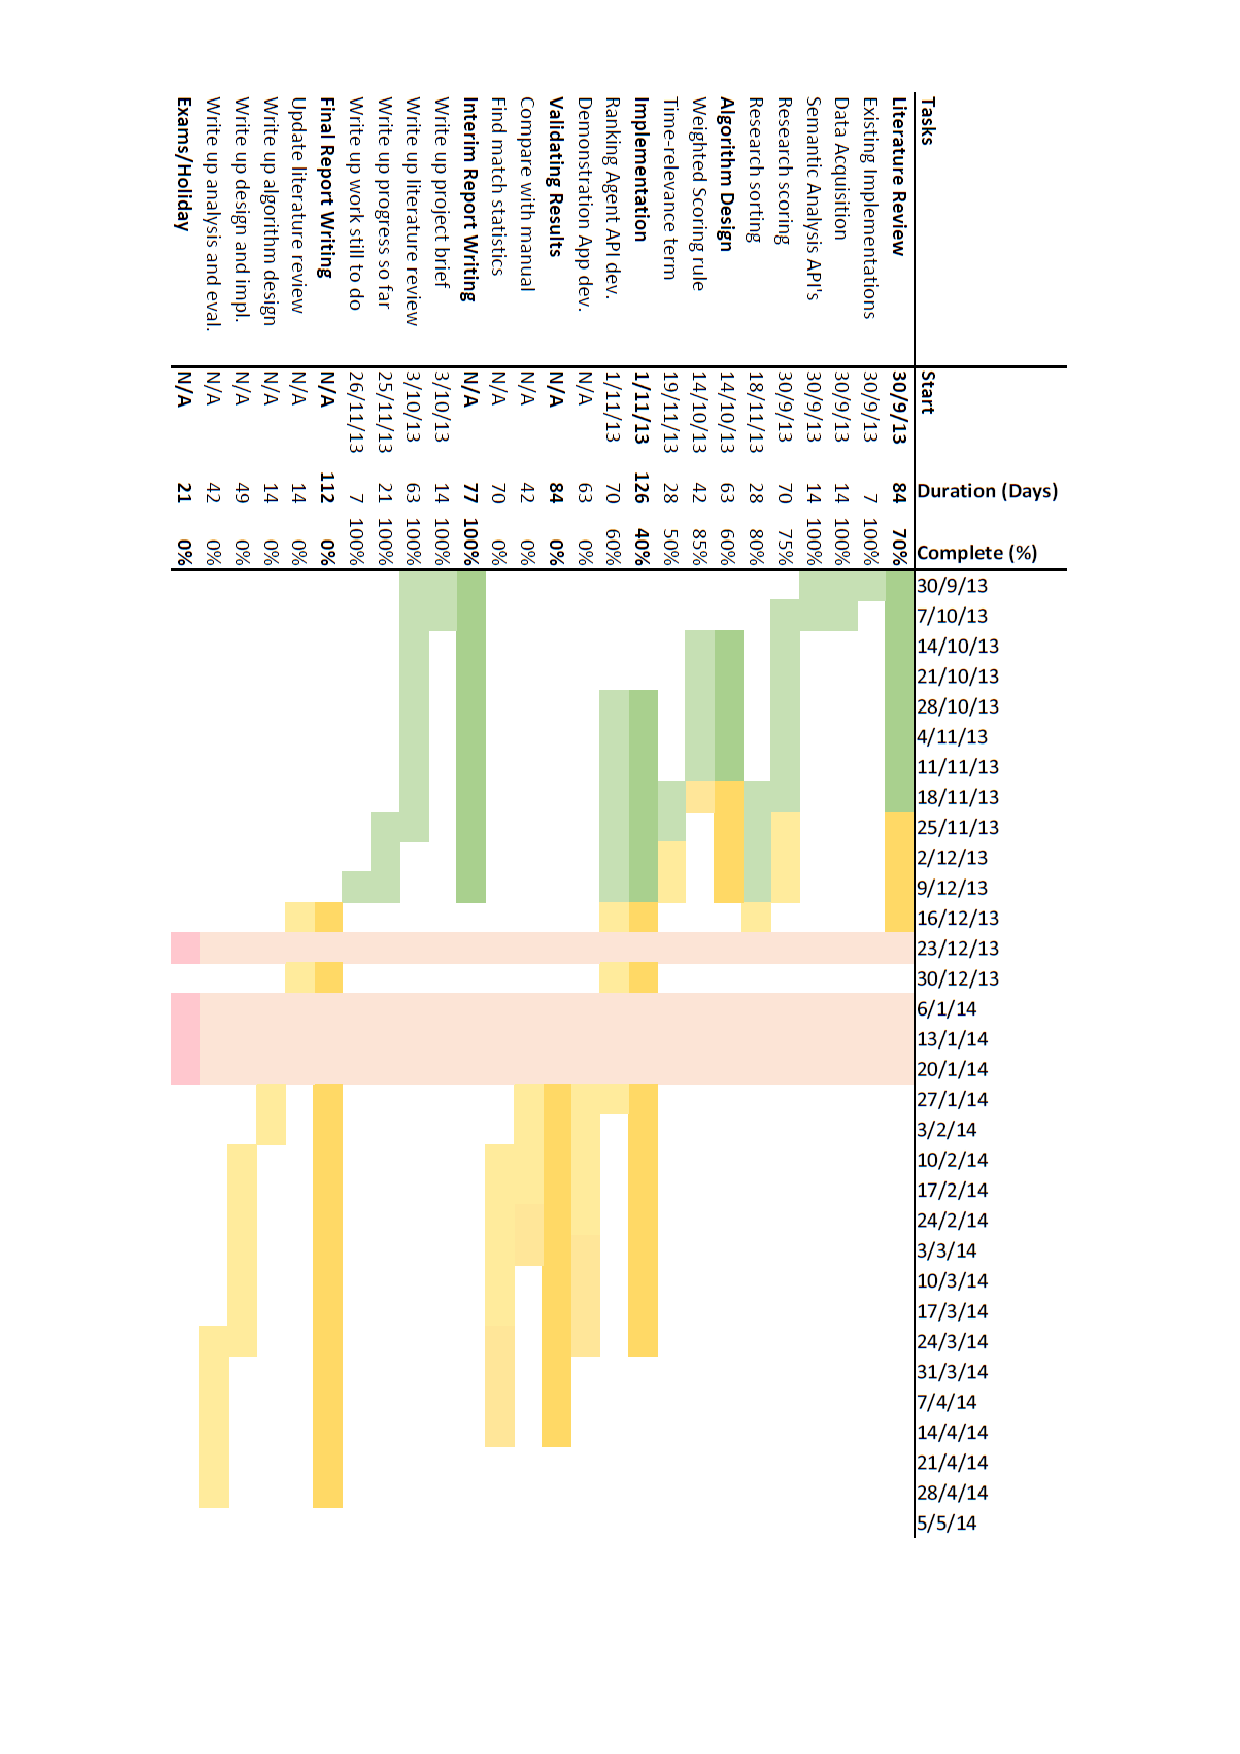
\includegraphics[width=1.3\linewidth]{images/gantt2.pdf}
    }
    \caption{Gantt Chart}
\end{figure}